\documentclass[aspectratio=169]{beamer}
\usetheme{Madrid}
\usecolortheme{default}
\usepackage[utf8]{inputenc}
\usepackage[T5]{fontenc}
\usepackage{graphicx}
\usepackage{hyperref}
\usepackage{booktabs}
\usepackage{amsmath}
\usepackage{listings}
\usepackage{color}

\definecolor{codegreen}{rgb}{0,0.6,0}
\definecolor{codegray}{rgb}{0.5,0.5,0.5}
\definecolor{codepurple}{rgb}{0.58,0,0.82}
\definecolor{backcolour}{rgb}{0.95,0.95,0.92}

\lstdefinestyle{mystyle}{
    backgroundcolor=\color{backcolour},   
    commentstyle=\color{codegreen},
    keywordstyle=\color{magenta},
    numberstyle=\tiny\color{codegray},
    stringstyle=\color{codepurple},
    basicstyle=\ttfamily\scriptsize,
    breakatwhitespace=false,         
    breaklines=true,                 
    captionpos=b,                    
    keepspaces=true,                 
    numbers=left,                    
    numbersep=5pt,                  
    showspaces=false,                
    showstringspaces=false,
    showtabs=false,                  
    tabsize=2
}
\lstset{style=mystyle}

\setbeamertemplate{caption}[numbered]
\renewcommand{\figurename}{Hình}
\renewcommand{\thefigure}{18.\arabic{figure}}

\title[Chương 18: Kỹ năng Thực chiến]{Học Sâu (Deep Learning) \\ \vspace{0.5cm} \Large Chương 18: Kỹ năng Thực chiến \& Tối ưu hóa Mô hình}
\author{Đại học Đông Á}
\date{\today}

\begin{document}

\begin{frame}
    \titlepage
\end{frame}

\begin{frame}{Nội dung chương}
    \tableofcontents
\end{frame}

\section{1. Tối ưu hóa Siêu tham số (Hyperparameter Tuning)}

\begin{frame}{Tham số và Siêu tham số}
    \begin{itemize}
        \item \textbf{Tham số (Parameters):} Là các trọng số (Weights) và độ lệch (Biases) mà mô hình tự động học được thông qua thuật toán Gradient Descent và Backpropagation.
        \item \textbf{Siêu tham số (Hyperparameters):} Là các thiết lập kiến trúc do con người định nghĩa trước khi huấn luyện. Ví dụ: Số lớp (layers), số node ẩn, Learning Rate, kích thước Batch, hàm Kích hoạt.
        \item \textbf{Vấn đề:} Không gian Siêu tham số không liên tục và không thể đạo hàm, do đó không thể dùng Gradient Descent để tối ưu.
    \end{itemize}
\end{frame}

\begin{frame}{Các chiến lược tìm kiếm Siêu tham số}
    \begin{itemize}
        \item \textbf{Grid Search (Tìm kiếm dạng lưới):} Duyệt qua mọi tổ hợp có thể của các siêu tham số. Tuyệt đối chính xác nhưng tốn thời gian theo cấp số nhân (Combinatorial Explosion).
        \item \textbf{Random Search (Tìm kiếm ngẫu nhiên):} Chọn ngẫu nhiên các tổ hợp trong không gian định sẵn. Nhanh hơn Grid Search và thường tìm được cấu hình đủ tốt trong thời gian ngắn.
        \item \textbf{Bayesian Optimization (Tối ưu hóa Bayes):} Sử dụng mô hình thống kê (Surrogate Model) để học từ các lần thử nghiệm trước, từ đó dự đoán tọa độ siêu tham số nào có khả năng cho ra kết quả tốt nhất ở lần thử tiếp theo.
    \end{itemize}
\end{frame}

\begin{frame}{Công cụ tự động hóa: KerasTuner}
    \begin{itemize}
        \item Trong thực tế, Kỹ sư Machine Learning không điều chỉnh siêu tham số bằng tay. Họ sử dụng thư viện tự động như \textbf{KerasTuner}.
        \item Quy trình hoạt động của KerasTuner:
        \begin{enumerate}
            \item Định nghĩa Không gian tìm kiếm (Search Space) (Ví dụ: Số lớp từ 2 đến 5, Learning rate $\{0.01, 0.001\}$).
            \item Xác định Hàm mục tiêu (Objective) (Ví dụ: \texttt{val\_accuracy} cao nhất).
            \item Chạy thuật toán dò tìm (Random Search, Hyperband, hoặc Bayesian Optimization).
            \item Lấy ra mô hình tốt nhất để triển khai.
        \end{enumerate}
    \end{itemize}
\end{frame}

\begin{frame}{Ứng dụng KerasTuner cho Kiến trúc SOTA}
    \begin{itemize}
        \item KerasTuner không chỉ tinh chỉnh các mạng đơn giản mà còn hỗ trợ không gian tìm kiếm được xây dựng sẵn cho các kiến trúc đỉnh cao (State-of-the-Art).
        \item Ví dụ: \texttt{kt.applications.HyperXception} và \texttt{kt.applications.HyperResNet}.
        \item Bằng cách sử dụng các mô hình Hyper này, hệ thống sẽ tự động tìm kiếm siêu tham số tối ưu trên nền tảng của ResNet và Xception mà không cần bạn phải tự thiết kế lại các khối Convolution phức tạp.
    \end{itemize}
\end{frame}

\begin{frame}[fragile]{Mã nguồn: Truy vấn cấu hình và Epoch tốt nhất}
\begin{lstlisting}[language=Python]
def get_best_epoch(hp):
    model = build_model(hp)
    callbacks = [
        keras.callbacks.EarlyStopping(
            # High patience to ensure convergence
            monitor="val_loss", mode="min", patience=10
        )
    ]
    history = model.fit(
        x_train, y_train, validation_data=(x_val, y_val),
        epochs=100, batch_size=128, callbacks=callbacks,
    )
    val_loss_per_epoch = history.history["val_loss"]
    best_epoch = val_loss_per_epoch.index(min(val_loss_per_epoch)) + 1
    return best_epoch
\end{lstlisting}
\end{frame}

\begin{frame}[fragile]{Mã nguồn: Huấn luyện mô hình siêu tham số tối ưu}
\begin{lstlisting}[language=Python]
def get_best_trained_model(hp):
    best_epoch = get_best_epoch(hp)
    model = build_model(hp)
    # Train on the full dataset without validation split
    model.fit(
        x_train_full, y_train_full, batch_size=128, epochs=int(best_epoch * 1.2)
    )
    return model

best_models = []
for hp in best_hps:
    model = get_best_trained_model(hp)
    model.evaluate(x_test, y_test)
    best_models.append(model)
\end{lstlisting}
\end{frame}

\begin{frame}{Rủi ro: Overfitting trên Validation Set}
    \begin{itemize}
        \item Việc tinh chỉnh Siêu tham số có một cạm bẫy cực kỳ nguy hiểm: \textbf{Quá khớp tập xác thực (Overfitting Validation Set)}.
        \item Vì ta luôn chọn những Siêu tham số đem lại kết quả tốt nhất trên tập Validation, ta đã vô tình biến tập Validation thành một dạng dữ liệu dùng để học.
        \item \textbf{Hậu quả:} Khi ra thực tế, mô hình sẽ hoạt động kém hơn mong đợi.
        \item \textbf{Giải pháp:} Luôn giữ lại một tập Test hoàn toàn độc lập (Không được dùng tập Test này để Early Stopping hay chọn KerasTuner).
    \end{itemize}
\end{frame}

\section{2. Suy diễn Đám đông - Model Ensembling}

\begin{frame}{Triết lý Ensemble: Suy diễn Đám đông}
    \begin{itemize}
        \item \textbf{Ensembling} (Tổ hợp mô hình) là kỹ thuật gộp dự đoán của nhiều mô hình khác nhau để tạo ra một dự đoán cuối cùng mạnh mẽ hơn.
        \item Triết lý: "Nhiều mô hình yếu cộng lại thành một mô hình mạnh".
        \item Dựa trên nguyên lý Thống kê: Nếu các mô hình có lỗi độc lập với nhau, sai số tổng thể sẽ triệt tiêu lẫn nhau.
        \item Điều này giống như câu chuyện "Thầy bói xem voi" - mỗi thầy bói chỉ sờ được một bộ phận, nhưng nếu họ họp lại và tổng hợp ý kiến, bức tranh toàn cảnh về con voi sẽ chính xác.
    \end{itemize}
\end{frame}

\begin{frame}[fragile]{Mã nguồn: Kỹ thuật Averaging (Trung bình hóa dự đoán)}
\begin{lstlisting}[language=Python]
# Uses four different models to compute initial predictions
preds_a = model_a.predict(x_val)
preds_b = model_b.predict(x_val)
preds_c = model_c.predict(x_val)
preds_d = model_d.predict(x_val)

# Simple average
# This new prediction array should be more accurate than any of the initial ones.
final_preds = 0.25 * (preds_a + preds_b + preds_c + preds_d)
\end{lstlisting}
\end{frame}

\begin{frame}[fragile]{Mã nguồn: Kỹ thuật Trung bình có Trọng số (Weighted Average)}
\begin{lstlisting}[language=Python]
# Not all models are equally good, so we weight them based on validation score
preds_a = model_a.predict(x_val)
preds_b = model_b.predict(x_val)
preds_c = model_c.predict(x_val)
preds_d = model_d.predict(x_val)

# These weights (0.5, 0.25, 0.1, 0.15) are assumed to be learned empirically.
final_preds = 0.5 * preds_a + 0.25 * preds_b + 0.1 * preds_c + 0.15 * preds_d
\end{lstlisting}
\end{frame}

\begin{frame}{Đa dạng hóa - Chìa khóa của Ensembling}
    \begin{itemize}
        \item Trong thuật toán tổ hợp, nếu ta kết hợp 5 mô hình giống hệt nhau, ta sẽ chẳng đạt được cải thiện nào.
        \item \textbf{Diversity (Đa dạng):} Các mô hình phải học từ những góc nhìn (Representations) khác nhau. Ví dụ: Kết hợp 1 CNN, 1 Transformer, và 1 Random Forest.
        \item \textbf{Bất đẳng thức Jensen:} Nếu hàm mất mát là hàm lồi (Convex), sai số của mô hình Ensemble luôn nhỏ hơn hoặc bằng trung bình sai số của các mô hình thành phần:
        $$ L(\mathbb{E}[M_i]) \leq \mathbb{E}[L(M_i)] $$
    \end{itemize}
\end{frame}

\section{3. Huấn luyện Phân tán (Distributed Training)}

\begin{frame}{Tại sao cần Huấn luyện phân tán?}
    \begin{itemize}
        \item Các mô hình SOTA (Ví dụ: LLMs, Vision Transformers) mất tới hàng chục nghìn năm để huấn luyện nếu chỉ dùng 1 GPU.
        \item Bằng cách nối mạng hàng nghìn GPU/TPU với nhau thành một cụm siêu máy tính (Cluster), thời gian huấn luyện giảm xuống chỉ còn vài tuần.
        \item Vấn đề cốt lõi: Làm sao chia việc cho hàng nghìn GPU chạy đồng thời mà không bị xung đột bộ nhớ và đảm bảo tiến trình Gradient cập nhật đúng?
    \end{itemize}
\end{frame}

\begin{frame}{Phân tán Dữ liệu vs Phân tán Mô hình}
    \begin{columns}
        \column{0.5\textwidth}
        \begin{itemize}
            \item \textbf{Data Parallelism:} Mỗi GPU chứa 1 bản sao y hệt của mô hình. Dữ liệu (Batch) được chẻ nhỏ ra (Ví dụ Batch 1024 chẻ thành 8 phần cho 8 GPU).
            \item \textbf{Model Parallelism:} Khi mô hình quá lớn không nhét vừa RAM 1 GPU, ta phải "chặt đứt" các Layer của mạng Nơ-ron và rải chúng ra nhiều GPU khác nhau.
        \end{itemize}
        
        \column{0.5\textwidth}
        \begin{figure}
            \centering
            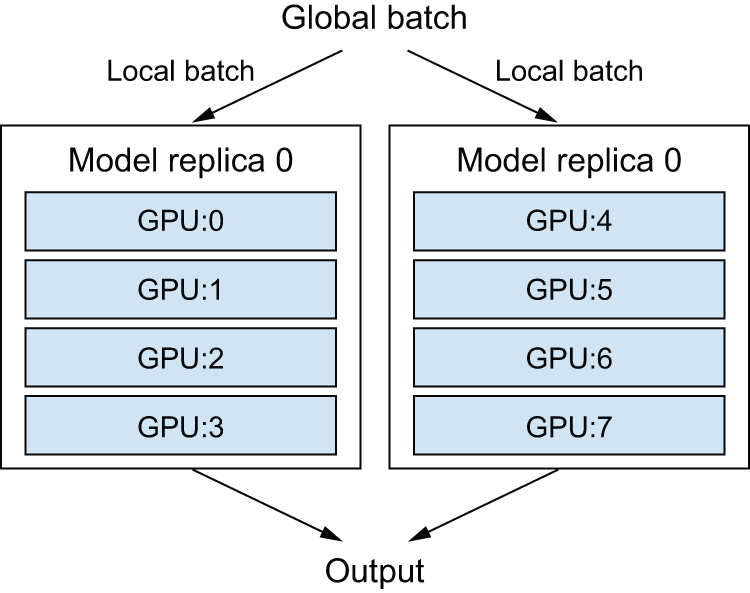
\includegraphics[width=\textwidth,height=0.6\textheight,keepaspectratio]{../../images/ch18/data_and_model_parallelism.1d1087a1.png}
            \caption{Sơ đồ hệ thống tính toán Phân tán hỗn hợp}
        \end{figure}
    \end{columns}
\end{frame}

\begin{frame}[fragile]{Mã nguồn: Khởi tạo Data Parallelism bằng JAX backend}
\begin{lstlisting}[language=Python]
import keras

# Get a list of available devices
# Example: ["gpu:0", "gpu:1", "gpu:2", "gpu:3"]
devices = keras.distribution.list_devices()

# Initialize Data Parallelism over all GPUs
keras.distribution.set_distribution(keras.distribution.DataParallel())

# Or over specific GPUs
keras.distribution.set_distribution(
    keras.distribution.DataParallel(["gpu:0", "gpu:1"])
)
\end{lstlisting}
\end{frame}

\begin{frame}{Đồng bộ hóa Gradient (All-Reduce Algorithm)}
    \begin{itemize}
        \item Trong Data Parallelism, nếu mỗi GPU nhận 1 tập dữ liệu con khác nhau, đạo hàm (Gradient) của chúng tính ra sẽ khác nhau.
        \item Nếu cập nhật trọng số trực tiếp, 8 GPU sẽ tự tạo ra 8 mô hình khác biệt hoàn toàn!
        \item \textbf{Đồng bộ (Synchronous Training):} Thuật toán All-Reduce ép tất cả GPU phải dừng lại vào cuối mỗi Step, truyền mạng gửi Gradient cho nhau, tính trung bình rồi mới thực hiện cập nhật cục bộ. Do đó, các GPU luôn có trọng số y hệt nhau.
    \end{itemize}
\end{frame}

\begin{frame}[fragile]{Mã nguồn: API DeviceMesh phân bổ hệ thống GPU}
\begin{lstlisting}[language=Python]
# We assume eight devices, organized as a 2 x 4 grid.
device_mesh = keras.distribution.DeviceMesh(
    shape=(2, 4),
    # It's convenient to give your axes meaningful names!
    axis_names=["data", "model"],
)

# You can also pass explicit devices
devices = [f"gpu:{i}" for i in range(8)]
device_mesh = keras.distribution.DeviceMesh(
    shape=(2, 4), axis_names=["data", "model"], devices=devices,
)
\end{lstlisting}
\end{frame}

\begin{frame}[fragile]{Mã nguồn: Phân vùng LayoutMap (Model Parallelism)}
\begin{lstlisting}[language=Python]
layout_map = keras.distribution.LayoutMap(device_mesh)
# None means "replicate the variable along this dimension."
# "model" means shard across the "model" axis of the device mesh.
layout_map["sequential/dense/kernel"] = (None, "model")
layout_map["sequential/dense/bias"] = ("model",)
layout_map["sequential/dense_1/kernel"] = (None, "model")
layout_map["sequential/dense_1/bias"] = ("model",)

model_parallel = keras.distribution.ModelParallel(
    layout_map=layout_map,
    batch_dim_name="data", # Axis named "data" handles data parallelism
)
keras.distribution.set_distribution(model_parallel)
\end{lstlisting}
\end{frame}

\begin{frame}[fragile]{Mã nguồn: Tối ưu hoá TPU (Tensor Processing Unit)}
\begin{lstlisting}[language=Python]
# TPUs are insanely fast but require large batch sizes to stay busy.
# If your dataset is small, cache it into memory to prevent IO bottleneck.
dataset = dataset.cache()

# Use "steps_per_execution" to fuse multiple steps into a single TPU run.
# This avoids the overhead of passing data back-and-forth to CPU.
model.compile(
    optimizer="adam",
    loss="sparse_categorical_crossentropy",
    steps_per_execution=8 # Run 8 batches per call
)
\end{lstlisting}
\end{frame}

\section{4. Tối ưu Bộ nhớ: Mixed-Precision \& Quantization}

\begin{frame}{Biểu diễn dấu phẩy động trong Khoa học Máy tính}
    \begin{columns}
        \column{0.5\textwidth}
        \begin{itemize}
            \item Máy tính lưu số thực IEEE 754 với 3 thành phần: Dấu (Sign), Số mũ (Exponent) và Định trị (Mantissa).
            \item Các giá trị được biểu diễn cách nhau một độ phân giải không đồng đều. Số càng lớn, khoảng cách giữa 2 số kế tiếp càng thưa.
            \item \textbf{Float32:} Dùng 32 bits. Chứa được dải giá trị rất chính xác, nhưng tiêu hao 4 bytes mỗi số.
            \item \textbf{Float16 \& Bfloat16:} Dùng 16 bits, tiết kiệm một nửa lượng RAM.
        \end{itemize}
        
        \column{0.5\textwidth}
        \begin{figure}
            \centering
            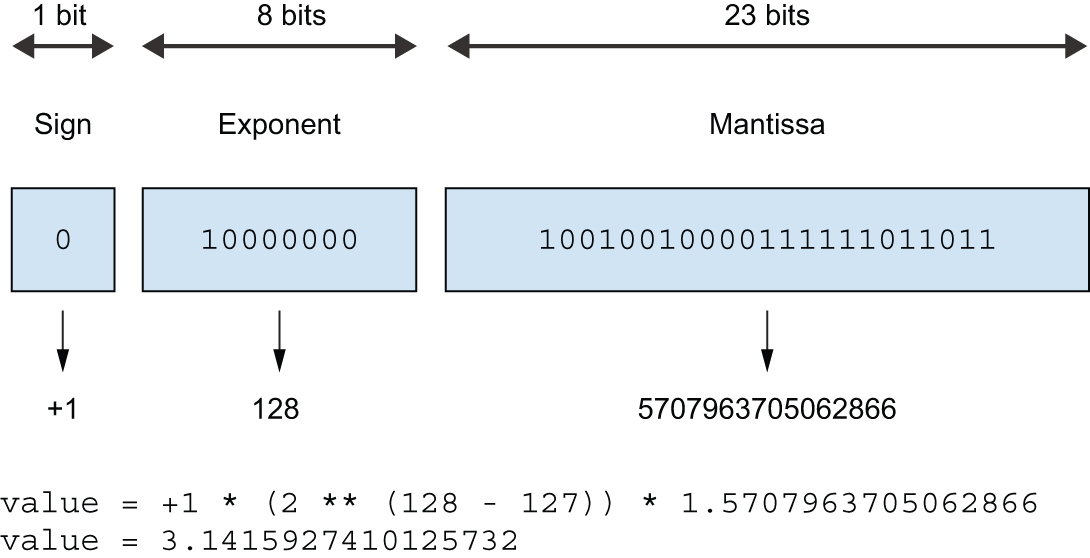
\includegraphics[width=\textwidth,height=0.6\textheight,keepaspectratio]{../../images/ch18/floating_pi.b6d4aaaf.png}
            \caption{Độ chính xác dấu phẩy động của số Pi}
        \end{figure}
    \end{columns}
\end{frame}

\begin{frame}{So sánh cấu trúc Float16 và Bfloat16}
    \begin{itemize}
        \item \textbf{Float16 (Half Precision):} Sử dụng 5 bits Số mũ và 10 bits Định trị. Rất chính xác cho các số nhỏ, nhưng dải biểu diễn tối đa dễ bị tràn số (Overflow).
        \item \textbf{Bfloat16 (Brain Float):} Sử dụng 8 bits Số mũ và 7 bits Định trị. Bhy sinh độ chính xác chi tiết (Mantissa) để mở rộng dải biểu diễn khổng lồ tương đương Float32. Bfloat16 hoạt động cực kỳ mượt trên TPU.
    \end{itemize}
    \begin{center}
    \begin{tabular}{lccc}
        \toprule
        \textbf{dtype} & \textbf{Bit ký hiệu} & \textbf{Bit số mũ} & \textbf{Bit Mantissa} \\
        \midrule
        \texttt{float16} & 1 & 5 & 10 \\
        \texttt{bfloat16} & 1 & 8 & 7 \\
        \texttt{float32} & 1 & 8 & 23 \\
        \bottomrule
    \end{tabular}
    \end{center}
\end{frame}

\begin{frame}[fragile]{Mã nguồn: Kích hoạt Float16 Inference}
\begin{lstlisting}[language=Python]
import keras

# Configure Keras to use float16 by default
# This provides nearly 2x speedup on modern GPUs/TPUs during predict()
keras.config.set_dtype_policy("float16")

# Alternatively, for TPUs, bfloat16 is usually better
keras.config.set_dtype_policy("bfloat16")
\end{lstlisting}
\end{frame}

\begin{frame}{Kỹ thuật Mixed-Precision Training}
    \begin{itemize}
        \item Trong lúc Training, nếu dùng \texttt{float16} $100\%$, giá trị Gradient (vốn rất nhỏ $\approx 10^{-6}$) sẽ bị làm tròn về số 0. Quá trình huấn luyện sụp đổ (Underflow).
        \item \textbf{Mixed-Precision:} Kết hợp ưu điểm của cả hai.
        \item \textbf{Forward \& Backward Pass:} Hệ thống ép kích hoạt xuống \texttt{FP16} để tăng tốc siêu hạng quá trình nhân ma trận (Matrix Multiplication).
        \item \textbf{Update Weights:} Master Weights được lưu trữ bằng \texttt{FP32} để cộng Gradient một cách an toàn.
    \end{itemize}
\end{frame}

\begin{frame}[fragile]{Mã nguồn: Kích hoạt Mixed-Precision trong Keras}
\begin{lstlisting}[language=Python]
import keras

# Turns on Mixed Precision Training automatically
keras.config.set_dtype_policy("mixed_float16")

# To prevent small gradients from rounding down to zero, we multiply the loss
# by a large constant scale factor (e.g. 1024.0) during Backpropagation.
optimizer = keras.optimizers.Adam(learning_rate=1e-3, loss_scale_factor=10)

# Better yet, let LossScaleOptimizer figure out the dynamic scaling automatically:
optimizer = keras.optimizers.LossScaleOptimizer(
    keras.optimizers.Adam(learning_rate=1e-3)
)
\end{lstlisting}
\end{frame}

\begin{frame}{Cấu hình Float8}
    \begin{itemize}
        \item Từ Float16, liệu ta có thể nén mô hình xuống \textbf{Float8} (8 bits)?
        \item Với Float8, tính toán sẽ sai số thảm họa nếu không có các kỹ thuật điều chỉnh Scale bù đắp. Keras chỉ hỗ trợ Float8 cho các lớp đặc thù của Transformer (Dense, EinsumDense, Embedding).
        \item Float8 thường chỉ hiệu quả với các dòng GPU cực mạnh (NVIDIA H100) và áp dụng cho các siêu mô hình Foundation Models ($>5$ Tỷ tham số).
    \end{itemize}
\end{frame}

\begin{frame}{Mất mát thông tin do Lượng tử hóa}
    \begin{itemize}
        \item Khi ép từ dải vô hạn của số thực xuống chỉ còn 256 giá trị của Int8, thông tin chắc chắn bị suy giảm.
        \item \textbf{Post-Training Quantization (PTQ):} Huấn luyện xong mô hình bằng Float32 rồi ép kiểu. Đơn giản, nhanh gọn nhưng giảm độ chính xác của mô hình.
        \item \textbf{Quantization-Aware Training (QAT):} Trong lúc huấn luyện Float32, hệ thống mô phỏng việc bị cắt cụt xuống Int8 ở quá trình Forward Pass. Do đó mô hình tự thích nghi với độ nhiễu lượng tử, giữ nguyên độ chính xác khi thực sự triển khai.
    \end{itemize}
\end{frame}

\begin{frame}{Lượng tử hóa (Quantization)}
    \begin{itemize}
        \item Để đưa các mô hình AI khổng lồ lên chạy trên Điện thoại hoặc IoT (Edge Devices) cho mục đích Suy diễn (Inference), ta phải nén chúng lại.
        \item \textbf{Quantization:} Ép kiểu các Trọng số từ số thực Float32 xuống số nguyên Int8. Giúp giảm 4 lần dung lượng RAM lưu trữ và chạy cực nhanh trên CPU.
        \item Thuật toán thường chia tỷ lệ dựa trên Max Absolute Value của phân phối. Các tham số sẽ nằm gọn trong khoảng số nguyên $[-127, 127]$.
    \end{itemize}
\end{frame}

\begin{frame}[fragile]{Mã nguồn: Mô phỏng thuật toán Abs-Max Lượng tử hoá INT8}
\begin{lstlisting}[language=Python]
from keras import ops

def abs_max_quantize(value):
    # Max of absolute value of the tensor
    abs_max = ops.max(ops.abs(value), keepdims=True)
    # Scale is max of int range (127) divided by max of tensor.
    scale = ops.divide(127, abs_max + 1e-7)
    
    scaled_value = value * scale
    # Rounding and clipping first is more accurate than directly casting.
    scaled_value = ops.clip(ops.round(scaled_value), -127, 127)
    
    # Casts to int8
    scaled_value = ops.cast(scaled_value, dtype="int8")
    return scaled_value, scale
\end{lstlisting}
\end{frame}

\begin{frame}[fragile]{Mã nguồn: API Int8 Quantization trong Keras}
\begin{lstlisting}[language=Python]
# Instantiates a trained model (or any quantizable layer like Transformer)
model = ...

# Boom! Compress the model.
model.quantize("int8")

# Now predict() and call() will run (partially) in int8!
# Very fast on CPU and takes 4x less RAM
predictions = model.predict(x_test)
\end{lstlisting}
\end{frame}

\section{5. Tổng kết: Vòng lặp Tiến bộ}

\begin{frame}{Vòng lặp Tiến bộ (The Loop of Progress)}
    \begin{columns}
        \column{0.5\textwidth}
        \begin{itemize}
            \item AI không bao giờ hoàn hảo ngay từ lần Train đầu tiên.
            \item Một kỹ sư Machine Learning phải liên tục thực thi vòng lặp: \textbf{Đánh giá} $\rightarrow$ \textbf{Phân tích lỗi} $\rightarrow$ \textbf{Tinh chỉnh ý tưởng} $\rightarrow$ \textbf{Huấn luyện lại}.
            \item Do đó, tối ưu Hệ thống (Multi-GPU, Mixed Precision) không chỉ để chạy cho vui, mà nó thu hẹp thời gian mỗi chu kỳ. Giúp ta tạo ra AI thông minh hơn trong cùng một quỹ thời gian.
        \end{itemize}
        
        \column{0.5\textwidth}
        \begin{figure}
            \centering
            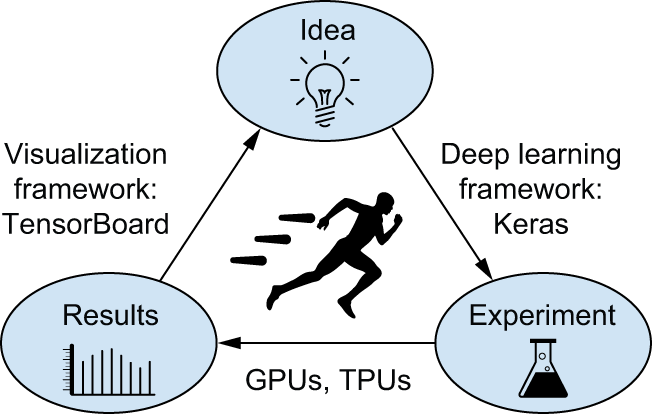
\includegraphics[width=\textwidth,height=0.6\textheight,keepaspectratio]{../../images/ch18/the_loop_of_progress.4bb26a08.png}
            \caption{Vòng lặp phát triển vô tận của ML}
        \end{figure}
    \end{columns}
\end{frame}

\begin{frame}{Tổng kết Khóa học}
    \begin{itemize}
        \item \textbf{Hyperparameter Tuning:} Dùng công cụ KerasTuner để tự động dò tìm kiến trúc, tránh điều chỉnh thủ công mù quáng.
        \item \textbf{Ensembling:} Áp dụng Bất đẳng thức Jensen và Suy diễn đám đông để đẩy hiệu suất mô hình vượt qua giới hạn của 1 mạng duy nhất.
        \item \textbf{Distributed Training:} Làm chủ Data Parallelism, DeviceMesh và LayoutMap JAX để thống trị phần cứng Data Center.
        \item \textbf{Memory Optimization:} Mix-Precision và Lượng tử hóa Int8 là yếu tố sống còn để đưa AI ra Sản phẩm thương mại (Production).
        \item \textbf{Kết thúc giáo trình:} Chúc mừng bạn đã hoàn thành giáo trình Học sâu hiện đại, từ Keras, ResNet, Transformer cho đến AI Sinh học. Chúc các bạn vững bước trên con đường AI Kỹ sư thực chiến!
    \end{itemize}
\end{frame}

\end{document}
